\chapter{Real-Time Analysis}

The best possible assignment for fixed prority is the Rate Monotonic and Deadline Monotonic assignement.\\
But how can I be sure that even using the optimal priority assignment, the schedule will meet all the deadlines?

This is the problem of \side{Real-Time analysis}: an activity that given a task set  and a scheduling policy, it responds to the query on whether or not the task set is schedulable.

What we have done so far is something very naive, i.e. simulating the schedule and verify that there is no deadline miss, but does not scale well in the case of long observation time of the system, until the schedule repeats itself. \\
Luckly there is a point/tme horizon, such that if no deadline miss happens withing this time horizon, you can certify none will occur ever after. How long is this time horizon depends:
\begin{itemize}
\item If there is no offset, we will find ourselves in the critical case, because if we have simultaneous activation of all the tasks in the task set, the system have an immediate request of computation time that needs to be satisfied.

In this case, it is sufficient  to simulate the schedule until the \side{hyperperiod}, i.e. the least common multiple of the periods
\[H = lcm\{T_i\}\]
This is because after the least common multiple of the period the task activation will be repeated.
\item If there is an offset, the schedule diagram can be shifted to meet the condition of the previous point.

Anyhow, given an offset
\[\phi_i = r_{i,}\]
it is necessary to simulate the schedule for at least 
\[2\,H + \phi_{max}\]
before being sure that the schedule will repeat itself.
\item If tasks periods are prime numbers the hyperperiod can be very large
\end{itemize}

Fortunately, there are better tests, that we can find, called \side{Utilisation Bound Analysis}.

\section{Utilisation-Based Analysis}
The Utilisation is the fraction of the processor that a task needs for its execution.

Hence, if a task have an activation time of $5$ and a computation time of 1, then its utilization is around $\sfrac{1/5}  = 20\%$.

So it would be nice to have a test that tells if a scheduling algorithm produces as feasible schedule simply based, on the utilisation bound.

A sufficient test  is based on the \side{Utilisation bound}:

The \side{utilisation least upper bound} for scheduling algorithm $\mathcal{A}$ is the smallest possible utilisation $U_{lub}$ such that, for any task set $\mathcal{T}$, if the task set's utilisation $U$ is not greater than $U_{lub}$ ($U\le U_{lub}$), then the task set is schedulable by algorithm $\mathcal{A}$

Formally:
\begin{itemize}
\item Each task uses the processor for a fraction of time, called worst case utilisation
\[U_i = \cfrac{C_i}{T_i}\]
\item The total processor utilisation is 
\[ U = \sum_i \,\cfrac{C_i}{T_i}\]
and it is a measure of the processor's load
\end{itemize}

One thing that we can immediately say is that if the total utiilisation exceed 100 \% there is no way that the task set is schedulable, i.e.
\[U > 1\qquad\text{taskset is not schedulable}\]
If the sum of all the utilisation is greater than 1/100\% we encounter a situation called stochastic instability, meaning that in the average you are asking the system more than it can offer.

In this case we have something similar since we have the worst case utilisation. In case the system requires more that it is available, there is no way the taskset is schedulable. Hence, this analysis yield a worst case guarantee.

Moreover, if $U < U_{lub}$ the taskset is schedulable. However:
\begin{itemize}
\item there is a ``gray area'' between $U_{lub}$ and 1, it depends on the specific performance of the algorithm under consideration.

So the ability of an algorithm to achieve a good utilisation bound is a measure of how efficient and effective the algorithm is.
\item We would like to have $U_{lub}$ close to 1.
\item $U_{lub} = 1$ would be optimal (hard upper bound, after 1 we are sure that the task set is not schedulable), it is physical impossible to outperform 100\% utilisation.
\end{itemize}

\subsection{Utilisation Bound for RM}
The notion of least upper bound can be described considering 2 tasks: one can make many choices of periods and computation times of the two tasks, taking the minimum value of $U$ below which all the task sets that I can choose are schedulable.\\
It can happen that some task that exceed the $U_{lub}$ is schedulable, but following the notion of least upper bound, as far as the task set is below this value the task set is guaranteed to be schedulable.

Formally: consider $n$ periodic (or sporadic) tasks with relative deadline equal to periods. The least upper bound for Rate Monotonic assignment can be obtained via the following expression:
\[U_{lub} = n(2^{\sfrac{1}{n}} - 1)\]
Note:
\begin{itemize}
\item $U_{lub}$ is a decreasing function of $n$
\item For large $n$: $U_{lub}\approx 0.69$
\end{itemize}

\begin{table}[!h]
\centering
\begin{NiceTabular}[hvlines]{c|c||c|c}
$\mathbf{n}$&$\mathbf{U}_{lub}$&$\mathbf{n}$&$\mathbf{U}_{lub}$\\
2 & 0.828 & 7&0.728\\
3 & 0.779 & 8 & 0.724\\
4 & 0.756 & 9 &0.720\\
5 & 0.743 & 10 & 0.717\\
6 & 0.734 & 11 & ...\\
\end{NiceTabular}
\end{table}

Therefore the schedulability test consists in:
\begin{enumerate}
\item Computing the utilisation
\[U = \sum_{i=1}^{n} \cfrac{C_i}{T_i}\]
\item If $U \le U_{lub}$, the task set is schedulable
\item If $U > 1$ the task set is not schedulable
\item If $U_{lub} < U \le 1$, the task set may or may not be schedulable
\end{enumerate}

\subsection{Utilisation Bound for DM}
In case of deadlines different from periods, one can always consider a conservative approximation in which the period is equal to the deadline. 

If relative deadlines are less than or equal to periods, instead of considering 
\[U = \sum_{i=1}^n \cfrac{C_i}{T_i}\]
we can consider:
\[U' = \sum_{i=1}^n \cfrac{C_i}{D_i}\]
Then the test is the same as the one for RM, except that we must use $U'$, instead of $U$.

And consequently:
\[\tau = (C,D,T)\,\rightarrow\,\tau' = (C,D,D)\]
If I can guarantee that this conservative approximation is schedulable than I can guarantee that the original task set is schedulable as well.

In summary:
\begin{itemize}
\item $\tau'$ is a \emph{worst case} for $\tau$
\item If $\tau'$ can be guaranteed, $\tau$ can be guaranteed too
\end{itemize}

\subsection{Pessimism}

The previously described condition is an extremely conservative approximation and most often than not the test would yield a non-schedulable result (above the least upper bound, even though the task set is schedulable).\\
The bound is very pessimistic: most of the times, a task set with $U > U_{lub}$ is schedulable by RM.

A particular case is when tasks have periods that are \side{harmonic}: a task set is harmonic, if for every two tasks $\tau_i, \tau_j$ either $T_i$ is multiple of $T_j$ or $T_j$ is multiple of $T_i$. In this case, and only in this case, the least upper bound of RM grows to1 (i.e. For a harmonic task set, the utilization bound is $U_{lub} = 1$).

In other words, Rate Monotonic is an optimal algorithm for harmonic task sets.

\section{Response Time Analysis}
So far with the utilisation bound we have seen that there is a sufficient schedulability condition: if the total utilisation is below the least upper bound than the system is schedulable. But this test works only if one makes very specific choices, i.e. to have the priority set using the RM assignment, otherwise the least upper bound does not apply.\\
Moreover, in the case in which the total utilisation is above the least upper bound, no conclusion can be drawn/no guarantees.

Therefore, we would like to utilize a \side{necessary and sufficient} test, which won't be analytical and nice as we have seen from an algorithmic point of view, but it will be a little more reliable since it requires to make much less assumptions.

Before introducing this test, let us recall the concept of response time: difference between the activation and the finishing/completion time. If one is able to compute the \side{worst-case response time} and if one can verify that such quantity remains below the \side{relative deadline}, then the system is schedulable.

The best thing about this test is that there is no assumption on the priority assignment, hence it can be applied to all algorithms. However, the periodic or sporadic tasks that we will be consider, are assumed to have no offsets (even though it is possible to have a variant of this analysis that applies).

Formally:
\begin{itemize}
\item For every task $\tau_i$ in the task set
\item Compute the worst case response time $R_i$ for $\tau_i$, i.e.
\[R_i = \max_j\{\rho_{i,j}\}\quad\text{with:}\,\,\rho_{i,j} = f_{i,j} - r_{i,j}\]
\item If $R_i \le D_i$, then the task is schedulable
\item Otherwise, the task is not schedulable
\end{itemize}

Consider a number of task set ordered by decreasing priority (i.e. $i < j \rightarrow p_i > p_j$) and consider no assumptions about the tasks offset (i.e. tasks can be activated at any time). We can define the \side{Critical Instant} as the most critical condition for the computation of the response time (if you allow the offset to change).

The obvious result is that if you allow the offset to change, the worst case situation in terms of response time (i.e. situation that produces the longest response time) is one in which all tasks start at the same time. Because if all the tasks start at the same time one would observe an utilisation peak.

Consider:
\begin{itemize}
\item a number of task set ordered by decreasing priority (i.e. $i < j\rightarrow p_i > p_j$) 
\item no assumptions about the tasks offset (i.e. tasks can be activated at any time)
\item the worst possible offsets combination
\end{itemize}

A job $J_{i,j}$ released at the \side{critical instant} experiences the maximum response time for $\tau_i$:
\[\forall k, \rho_{i,j} \ge \rho_{i,k}\]
\begin{theorem}
The critical instant for task $\tau_i$ occurs when job $J_{i,j}$ is released at the same time with a job in every high priority task.
\end{theorem}
Hence if all the offsets are 0, the first job of every task is released at the critical instant.

How one can compute the worst case response time?
The worst case response time $R_i$ for task $\tau_i$ depends on:
\begin{itemize}
\item Its execution time
\item The execution time of higher priority tasks (since the higher priority tasks can \side{preempt} task $\tau_i$ and increase its response time), aka \side{scheduling interference}.

This factor is given by the number of activations of the higher priority tasks, in the window from the critical instant to the response time times the execution time/computation time of the higher priority tasks.
\end{itemize}
as a consequence, the worst case response time can be computed as:
\[R_i = C_i + \sum_{h=1}^{i-1}\,\ceil{\cfrac{R_i}{T_h}}\,C_h\]
Unfortunately, one can notice that the above expression in recursive/\side{implicit equation} + nonlinear given the presence of the ceiling operator (i.e. $R_i = f(R_i)$), as a consequence, there is no closed-form expression for computing the worst case response time $R_i$.

We need an iterative method to solve the equation.

\begin{figure}[!h]
\centering
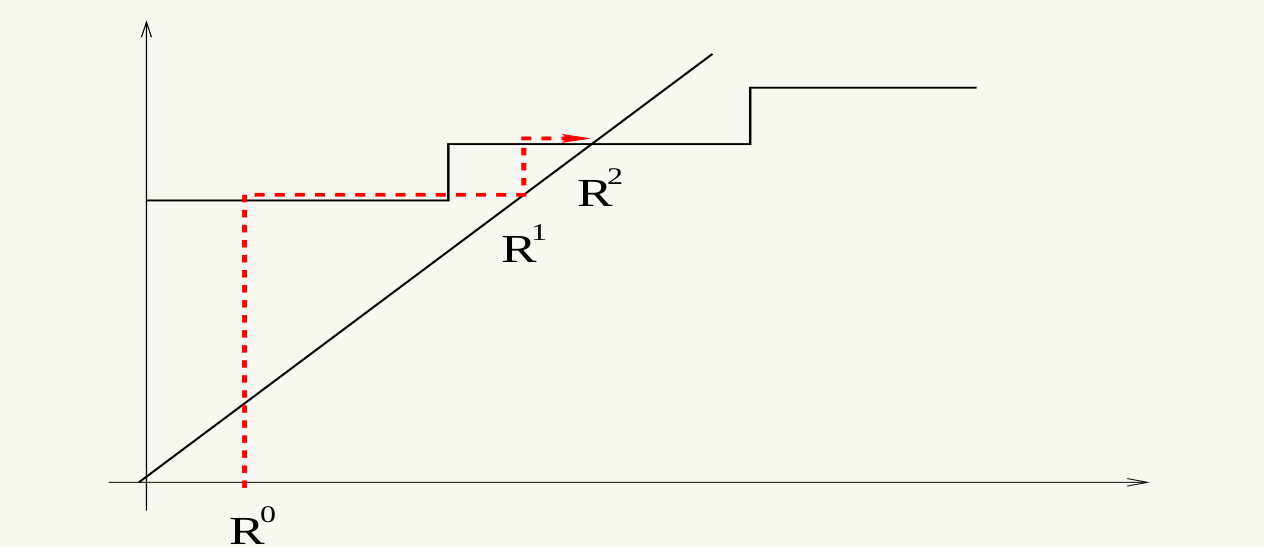
\includegraphics[width=.8\textwidth]{image05}
\end{figure}
The point where the \side{bisector} intersects the stairway, is the solution to the equation. But how one can find such intersection?\\
In terms of algorithms it means that, one have a first guess which is

\begin{itemize}
\item Iterative solution:
\[R_i = \lim_{k\to\infty} R_i^{(k)}\]
where $R_i^{(k)}$ is the worst case response time for $\tau_i$ at step $k$
\item Hence, we can start from a first estimation of the response time:
\[R_{i}^{(0)} = C_i\]
\item Compute the interference in this interval
\[R_{i}^{(1)} = C_i + \sum_{h=1}^{i-1}\ceil{\cfrac{R_{i}^{(0)}}{T_h}} C_h\]
Since all the tasks starts at the same instant (critical instant), I am sure that I would have at least one activation, hence
\[R_i^{(0)} = C_i + \sum_{h=1}^{i-1} C_h\]
\item Repeat the iterative step:
\[R_{i}^{(1)} = C_i + \sum_{h=1}^{i-1}\ceil{\cfrac{R_{i}^{(k-1)}}{T_h}} C_h\]
\item The iteration stops when:
\begin{itemize}
\item $R_i^{(k+1)} = R_i^{(k)}$
\item $R_i^{(k)} > D_i$ (non schedulable)
\end{itemize}
\end{itemize}

This is a standard method to solve non-linear equations in an iterative way. If a solution exists (the system is not overloaded, i.e. total utilisation of the task is below 1), $R_i^{(k)}$ converges to it, otherwise the failing condition avoids infinte iterations.

\subsection{Considerations}
\begin{enumerate}
\item The response time analysis is an efficient algorithm
\item In the worst case the number of steps $N$ for the algorithm to converge is exponential
\item depends on the total number of jobs of higher priority tasks in the interval $[0, D_i]$
\[N \propto \sum_{h=1}^{i-1}\ceil{\cfrac{D_h}{T_h}}\]
\item If $s$ is the minimum granularity of the time, then in the worst case 
\[N = \cfrac{D_i}{s}\]
\item However, such worst case is very rare: usually, the number of steps is low.
\end{enumerate}


There are a few corner case conditions:

Suppose you have three tasks:
\[\tau_1 = (1,4,4)\qquad \tau_2 = (2,6,6)\qquad \tau_3 = (1,8,8)\]
This task set is schedulable, however, the slack for the last task is too large and too much time is spent being idle.

There is an high discontinuity of the response time, in fact, one can easily construct examples in which, this condition can bring the system to a critical failure. To be precise: a small variability in the computation time can cause and high variability in the response time (due to preemption of low priority tasks) and occasionally cause deadline misses (\side{domino effect}: if you deviate too much from the nominal condition this might result in deadline misses).

The worst case response time is a metric that is very much used to assess the feasibility of the schedule but it cannot be used to assess the \side{robustness of a scheudulability condition}.\\
Consequenlty, he slack (time it takes to reach the deadline) is by no means a measure of how much robust your system is.


\section{Time Demand Analysis}

It is very similar to response time analysis apart from some critical differences that make it so while the \side{time demand analysis} does not give you any information on the delays introduced by a computation, it does give you information about the \side{robustness of a schedule}.

Both time demand analysis and response time analysis equally based on necessary and sufficient conditions, equally well founded, that provides you with a different type of information
\begin{itemize}
\item Response time analysis does not only tell you if a task set is schedulable or not but it also tells you what are the delays introduced in the computation
\item Time demand analysis does not give you any information about the delays introduced in the computation but  it gives you information on the sensibility/robustness of the result
\end{itemize}

Processor Demand approach has been proposed by Lehoczky and others in 1989 and later refined by Audsley and other in 1993 and by Baruah in 1990. The concept is very simple: in any interval, the computation demanded by all tasks in the set must never exceed the available time.
\begin{itemize}
\item First and foremost we need to consider an interval in which we compute the computation demanded by all the tasks in this interval\item If there is an instant before the deadline in which the total computation time demanded by the task is matched by the offer of the computation time of the processor, then we reached a point where we have exhausted all the backlog and we can say that the system is schedulable.
\item The problem is: how to compute the time demanded by a task set $\mathcal{T}$?

We can exploit the key obseration of critical instant and all the offsets are set to 0 (this allows us to only consider the first job of each task).
\end{itemize}

Given an interval $[t_1, t_2]$, let $\mathcal{J}_{t_1,t_2}$ be the set of jobs started after $t_1$ and with deadline lower that or equal to $t_2$:
\[\mathcal{J_{t_1, t_2}} = \{J_{i,j}: r_{i,j} \ge t_1 \wedge d_{i,j} \le t_2\}\]
In other terms, this subset is the collection of jobs that needs to be offered within the interval $[t_1, t_2]$.

Moreover we can define the \side{processor demand} in $[t_1, t_2]$ as:
\[W(t_1, t_2) = \sum_{J_{i,j}\in\mathcal{J}_{t_1,t_2}}c_{i,j}\]
In other terms, is the sum of the computation times of all the jobs that have been activated and completed within the specified interval.

In this case, the lower case signifies the theoretical possibility of each job to have a different computation time. However, in practice we will consider the WCET $C_i$ instead of $c_{i,j}$.

The computation demanded in every interval $[t_1, t_2]$, has to be smaller than the lenght of the interval (computation time offered by the CPU)
\[W(t_1, t_2) \le t_2-t_1\qquad\forall(t_1,t_2)\]
In theory, we should consider the hyperperiod and make $t_1$ and $t_2$ change and repeat the check for every combinations.

In practice, a first simplification is not considering the whole period given that this analysis can be done for each task.
And for each task you can consider only the first job. Because the first job is the one affected by the highest computation time (cfr. critical instant).

Hence, if the first job of a task succeeds in satisfying this constraint we are in a good shape. There will not be another job in which the computation demanded by the old task system would be higher.

Clearly for a task you need to consider in the computation demand not the entire task set but only the computation demand of the task itself + the demand of the tasks having higher priority. Formally:

$W_i(t_1, t_2)$ is the time demanded in $[t_1, t_2]$ by all tasks $\tau_j$ with $p_j \ge p_i$ ($\Rightarrow j \le i$).

As mentioned:
\begin{itemize}
\item We can consider only $W_i(0, t)$, i.e. from the critical instant
\item For task $\tau_i$, only check $W_i(0,t )$ for $0\le t\le D_i$
\item It can be shown that we can change the universal quantifier $\forall$ into the existential quantifier $\exists$. 

If you consider a task $\tau_i$, what is the number of jobs originated by it in the interval $[0, t]$? 
\[\floor{\cfrac{t}{T_i}}\]
If instead we use the ceil instead the floor, we are making a conservative approximation (overevaluation), but this overevaluation allows us to swap the two quantifiers.
\item We can therefore say if there is an instant in which this overevaluation/overestimation is matched by the offer than we are ok-

\[W_i(0,t) = C_i + \sum_{h=1}^{i-1}\ceil{\cfrac{t}{T_h}}\,C_h\]
\end{itemize}

We have obtained a function is a stairway and we have to look for a point in which $W_i(0,t) < t$.

\subsection{The Guarantee}
The Task $\tau_i$ is schedulable iff $\exists t: 0\le t\le D_i \wedge W_i(0,t) \le t$.

A task set $\mathcal{T}$ is schedulable iff:
\[\forall \tau_i \in \mathcal{T}, \exists t: 0 \le t \le D_i \wedge W_i(0, t) \le t\]
Sometimes, different notations in literature
\[W_i(0,t) \rightarrow W_i(t) =\sum_{h=1}^{i}\ceil{\cfrac{t}{T_h}}C_h\]
implying that one of the extreme is zero.

Someone defines
\begin{gather*}
L_i(t_1, t_2) = \cfrac{W_i(t_1, t_2)}{t_2 - t_1}\\
L_i = \min_{0\le t\le D_i} L_i(0,t) \qquad L = \max_{\tau_i\in\mathcal{T}} L_i
\end{gather*}
The guarantee tests then becomes: 
Task $\tau_i$ is schedulable iff $L_i \le 1$.\\
$\mathcal{T}$ is schedulable iff $L \le 1$.

\subsection{Simplifications}
The test might still be long (need to check many values of $L(0, t)$ to find the minimum).

The number of points to check for computing $\sfrac{W_i}{L_i}$ can be reduced by considering the so called \side{scheduling points}: i.e. points in which the stairways changes value.

Formally, the scheduling points are mathematically defined as:
\[S_i = \{k\,T_h | h \le i; 1 \le k \le \floor{\cfrac{T_i}{T_h}}\}\]
hence the number of scheduling points is a multiple of $T_h$ for $h \le i$, and the test can be rewritten in the simplified way:
\[L_i = \min_{t\in S_i} L_i(0,t)\]

To be fair, we have to say that this si even too much, because it can be shown that some of these scheduling points dominate the others: there is a selection of scheduling points to which you can restrict your analysis.

 














